% Template for IGARSS-2018 paper; to be used with:
%          spconf.sty  - LaTeX style file, and
%          IEEEbib.bst - IEEE bibliography style file.
% --------------------------------------------------------------------------
\documentclass{article}
\usepackage{spconf,amsmath,epsfig,graphicx}
\usepackage{subcaption}

% Example definitions.
% --------------------
\def\x{{\mathbf x}}
\def\L{{\cal L}}

% Title.
% ------
\title{Unsupervised Sequential Classification of MODIS Time-Series}
%
% Single address.
% ---------------
\name{T.L. Grobler$^{\dagger}$, W. Kleynhans$^{\star}$ and B.P. Salmon$^{\ddagger}$}
\address{$\dagger$Dept of Mathematical Sciences, Computer Science Division, Stellenbosch University,\\ Private Bag X1, 7602 Matieland, South Africa\\
$\star$Department of Electrical, Electronic and Computer Engineering University of Pretoria,\\
Pretoria 0002, South Africa\\
${\ddagger}$School of Engineering, University of Tasmania,
Hobart, TAS 7001, Australia}
%
% For example:
% ------------
%\address{School\\
%	Department\\
%	Address}
%
% Two addresses (uncomment and modify for two-address case).
% ----------------------------------------------------------
%\twoauthors
%  {A. Author-one, B. Author-two\sthanks{Thanks to XYZ agency for funding.}}
%	{School A-B\\
%	Department A-B\\
%	Address A-B}
%  {C. Author-three, D. Author-four\sthanks{The fourth author performed the work
%	while at ...}}
%	{School C-D\\
%	Department C-D\\
%	Address C-D}
%
\begin{document}
%\ninept
%
\maketitle
%
\begin{abstract}
In this paper we present a class label agnostic dimensionality reduction comparison framework. 
We illustrate the usefulness of this framework at the hand of a case study. For our case study, we consider two prominent land cover classes in the Gauteng province, namely natural vegetation and settlement using an 8 year MODIS dataset. We use the framework to compare two 
feature extraction techniques, namely PCA and FFT. For the case study we considered in this paper, the PCA technique produced a reduced feature space which was 15\% more 
separable than the feature space produced by the FFT method.
\end{abstract}
%
\begin{keywords}
Principal Component Analhysis (PCA), harmonic analysis, hypertemporal remote sensing.
\end{keywords}
%

\section{Introduction}
\label{sec:intro}
Hallo \cite{almeida2015}.

\begin{minipage}[b]{.47\linewidth}
  \centering 
  \centerline{\epsfig{figure=11.pdf,width=4.0cm}}
  %\vspace{1.5cm}
  \centerline{(a) Band 1}\medskip
\end{minipage}
\hfill
\begin{minipage}[b]{0.47\linewidth}
  \centering
  \centerline{\epsfig{figure=22.pdf,width=4.0cm}}
  %\vspace{1.5cm}
  \centerline{(b) Band 2}\medskip
\end{minipage}

\begin{minipage}[b]{.47\linewidth}
  \centering 
  \centerline{\epsfig{figure=33.pdf,width=4.0cm}}
  %\vspace{1.5cm}
  \centerline{(c) Band 3}\medskip
\end{minipage}
\hfill
\begin{minipage}[b]{0.47\linewidth}
  \centering
  \centerline{\epsfig{figure=44.pdf,width=4.0cm}}
  %\vspace{1.5cm}
  \centerline{(d) Band 4}\medskip
\end{minipage}


\begin{figure*}[h] 
  \begin{subfigure}[b]{0.49\linewidth}
    \centering
    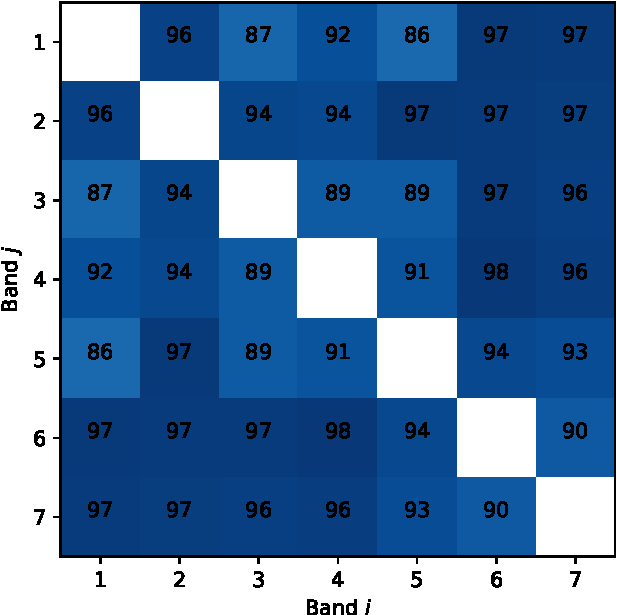
\includegraphics[width=0.9\linewidth]{sup-crop.pdf} 
    \caption{Logarithm applied} 
    \label{fig7:a} 
    %\vspace{4ex}
  \end{subfigure}%% 
  \begin{subfigure}[b]{0.49\linewidth}
    \centering
    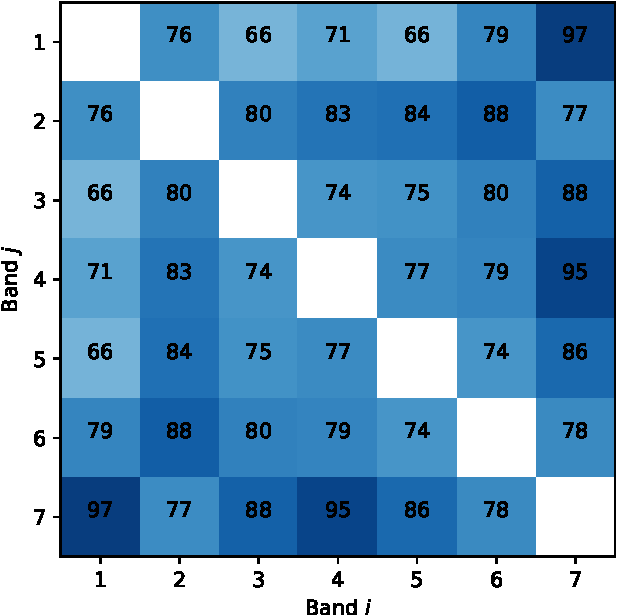
\includegraphics[width=0.9\textwidth]{un-crop.pdf} 
    \caption{Binary segmented image} 
    \label{fig7:b} 
    %\vspace{13ex}
    \end{subfigure} 
  \begin{subfigure}[b]{0.49\linewidth}
    \centering
    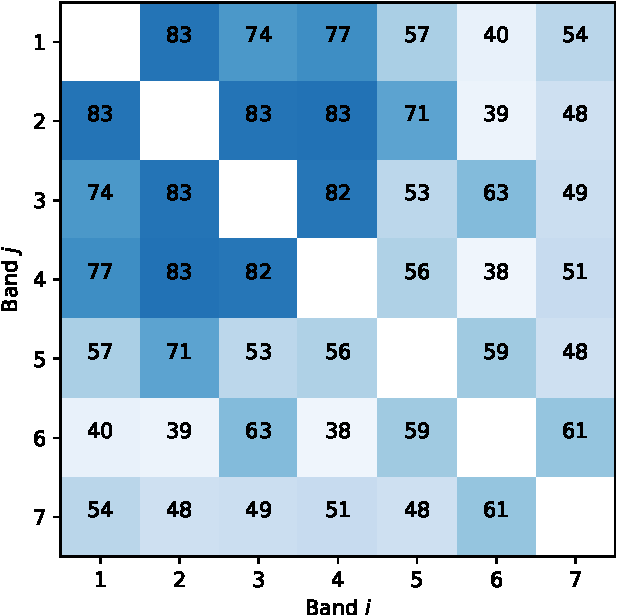
\includegraphics[width=0.9\textwidth]{kmeans-crop.pdf} 
    \caption{Hough Transform} 
    \label{fig7:c} 
  \end{subfigure}%%
  \begin{subfigure}[b]{0.49\linewidth}
    \centering
    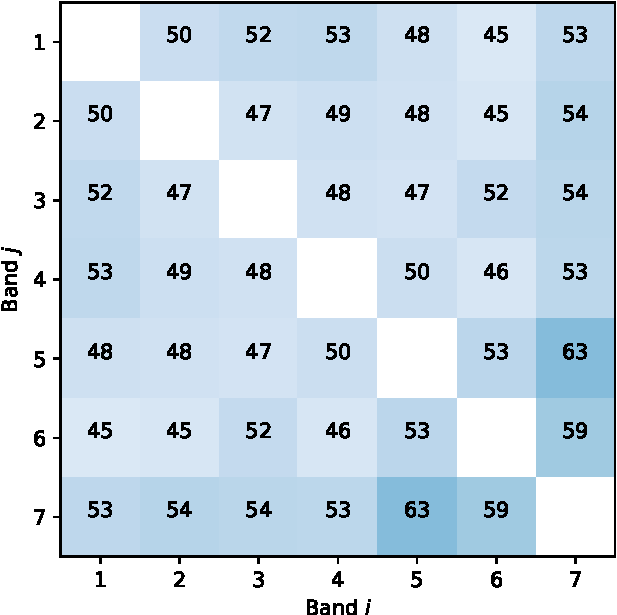
\includegraphics[width=0.9\textwidth]{gmm-crop.pdf} 
    \caption{Segmented image} 
    \label{fig7:d} 
  \end{subfigure} 
  \caption{c}
  \label{fig7} 
\end{figure*}





\section{Conclusion}
\label{sec:ref}
We presented a label agnostic feature extraction comparison framework in this paper. We demonstrated its usefulness by employing it and a case study to compare two feature extraction methods,
namely FFT and PCA (we also found that the PCA approach outperformed the FFT approach).

%List and number all bibliographical references at the end of the paper.  The references can be numbered in alphabetic order or in order of appearance in the document.  When referring to them in the text, type the corresponding reference number in square brackets as shown at the end of this sentence \cite{C2}.

% References should be produced using the bibtex program from suitable
% BiBTeX files (here: strings, refs, manuals). The IEEEbib.bst bibliography
% style file from IEEE produces unsorted bibliography list.
% -------------------------------------------------------------------------
\bibliographystyle{IEEEbib}
\bibliography{strings,refs}

\end{document}
